\begin{algorithm*}[tb]
   \caption{Iterative Refinement}
   \label{alg:example}
\begin{algorithmic}
   \STATE {\bfseries Input:} Original data $D$ with $x$ and $y$,
   \STATE $D_{+} \gets D $ 
   \STATE $D_{pref} \gets \{\} $ 
   \STATE $\theta_O = FT(y | x)$ where $x , y \sim D $ 
   \FOR{$j=1$ {\bfseries to} $M$}
    \STATE $y_j \gets p_{\theta_{j-1}}(x)$  
    \COMMENT{Generate candidate answers}
    \STATE $y_j^{+} , y_j^{-} \gets Oracle(y_j, y)$
    \COMMENT{Categorize to correct and incorrect set}
    \STATE $y_j^{+} , y_j^{-} \gets Filter(y_j^{+} , y_j^{-})$
    \STATE $D_{+} \gets D_{+} \cup (x,y_j^{+}) $
    \STATE $D_{pref} \gets D_{pref} \cup (x,y_j^{+}, y_j^{-}) $
    \STATE $D_{+} \gets Filter_{\Omega_{j-1}}(D_{+})$
    \STATE $D_{pref} \gets Filter_{\Omega_{j-1}}(D_{pref})$
    \STATE $\theta_J = FT(y | x)$ where $x , y \sim D_+ $
    \STATE $\Omega_J = DPO(y^{+} , y^{-}  | x)$ where $x , y^{+} , y^{-} \sim D_{pref} $

   \ENDFOR
\end{algorithmic}
\end{algorithm*}



Generating from a language model involves sampling from the most likely tokens, one at a time. Due to this limitation, LLMs are prone to hallucination and inconsistency as there is no limitation that guarantees the correctness of a whole generated text. And yet, LLMs can be prompted to reason logically e.g. ``Let's think step-by-step'' \citep{wei_chain--thought_2022} so recent work has aimed to improve formal reasoning so that LLMs may be logically self-consistent in their responses. The modern approach has been finetuning on high-quality reasoning dataset e.g. mathematical problems \citep{cobbe_training_2021} where the correct answer is provided. But LLMs can still learn to answer correctly while reasoning incorrectly \citep{lightman_lets_2023}, learning bad reasoning and hindering their ability to generalize. The challenge becomes how to guide LLM reasoning. Initial approaches were naive: supervised finetuning on the answer given the question.

Next, researchers showed that prompting and few-shot examples could improve performance \citep{wei_chain--thought_2022} and generating a rationale i.e. logical reasoning steps before answering is key \citep{lightman_lets_2023}. But datasets only include the correct final answer, not the correct rationale as it is too expensive to manually generate. So \citet{zelikman_star_2022} generated rationales from an LLM and marked it correct if it leads to the right answer. But then models could still learn the right answer for the wrong reasons. This motivated the learning of two models: a generator and a verifier \citep{cobbe_training_2021, lightman_lets_2023}, where the generator is trained to produce logical steps and an answer, as previously, and the verifier is trained to distinguish between a correct and incorrect rationale. At test time, the verifier is used to rank multiple guesses from the generator to pick the best one. We propose to iterate between learning the generator and learning the verifier to improve both and lead to models with better reasoning skills.


\begin{figure}[ht]
\vskip 0.2in
\begin{center}
\centerline{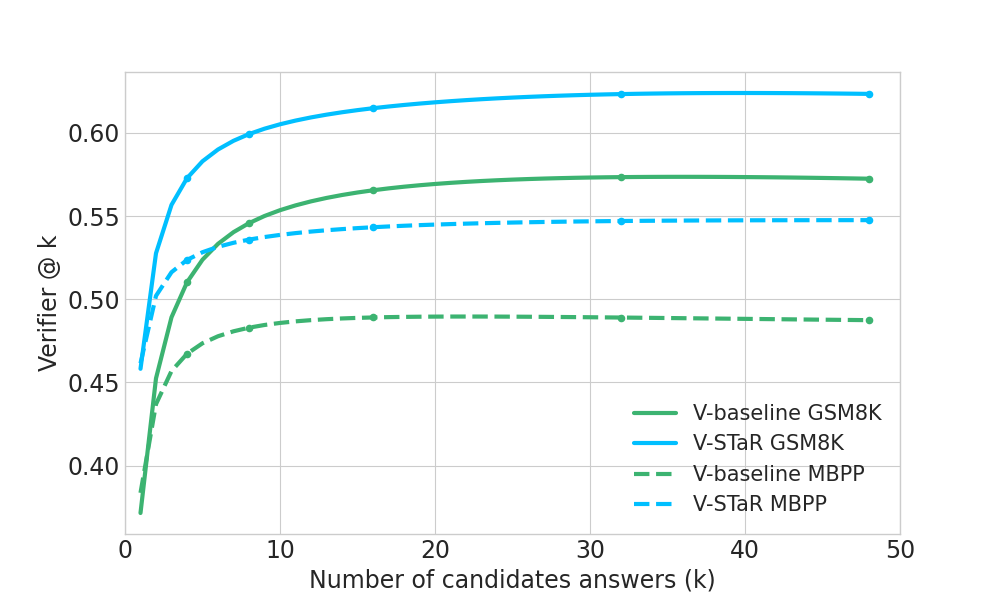
\includegraphics[width=\textwidth/2]{icml2023/figs/ver_at_k.png}}
\caption{}
\label{algo}
\end{center}
\vskip -0.2in
\end{figure}



\begin{figure}[ht]
\vskip 0.2in
\begin{center}
\centerline{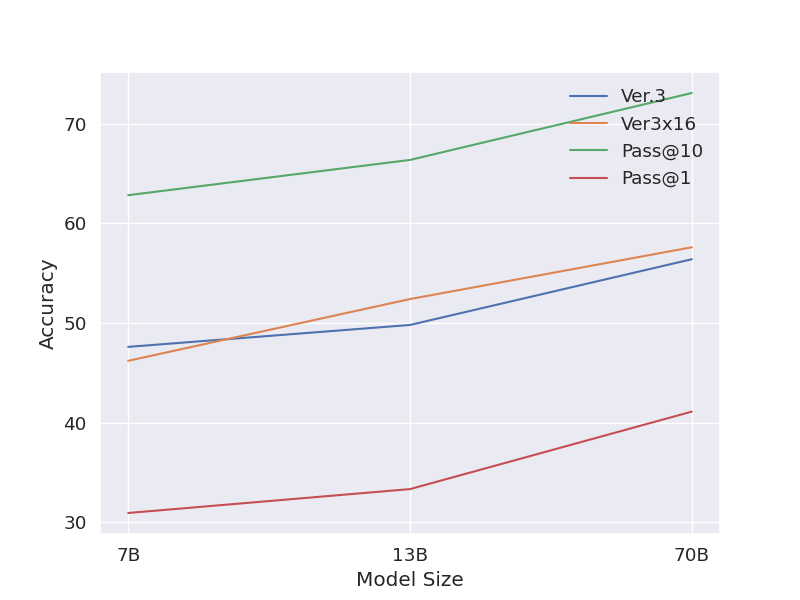
\includegraphics[width=\textwidth/2]{icml2023/figs/mbpp_verifier_transfer.png}}
\caption{MBPP Verifier transfer performance}
\label{mbpp_ver_transfer}
\end{center}
\vskip -0.2in
\end{figure}


\begin{figure}[ht]
\vskip 0.2in
\begin{center}
\centerline{\includegraphics[width=\textwidth/2]{icml2023/figs/cross_verifier_heatmap.png}}
\caption{Cross evaluation of verifiers and generators of different iterations.}
\label{ver_cross}
\end{center}
\vskip -0.2in
\end{figure}

\begin{figure*}[ht]
\vskip 0.2in
\begin{center}
\centerline{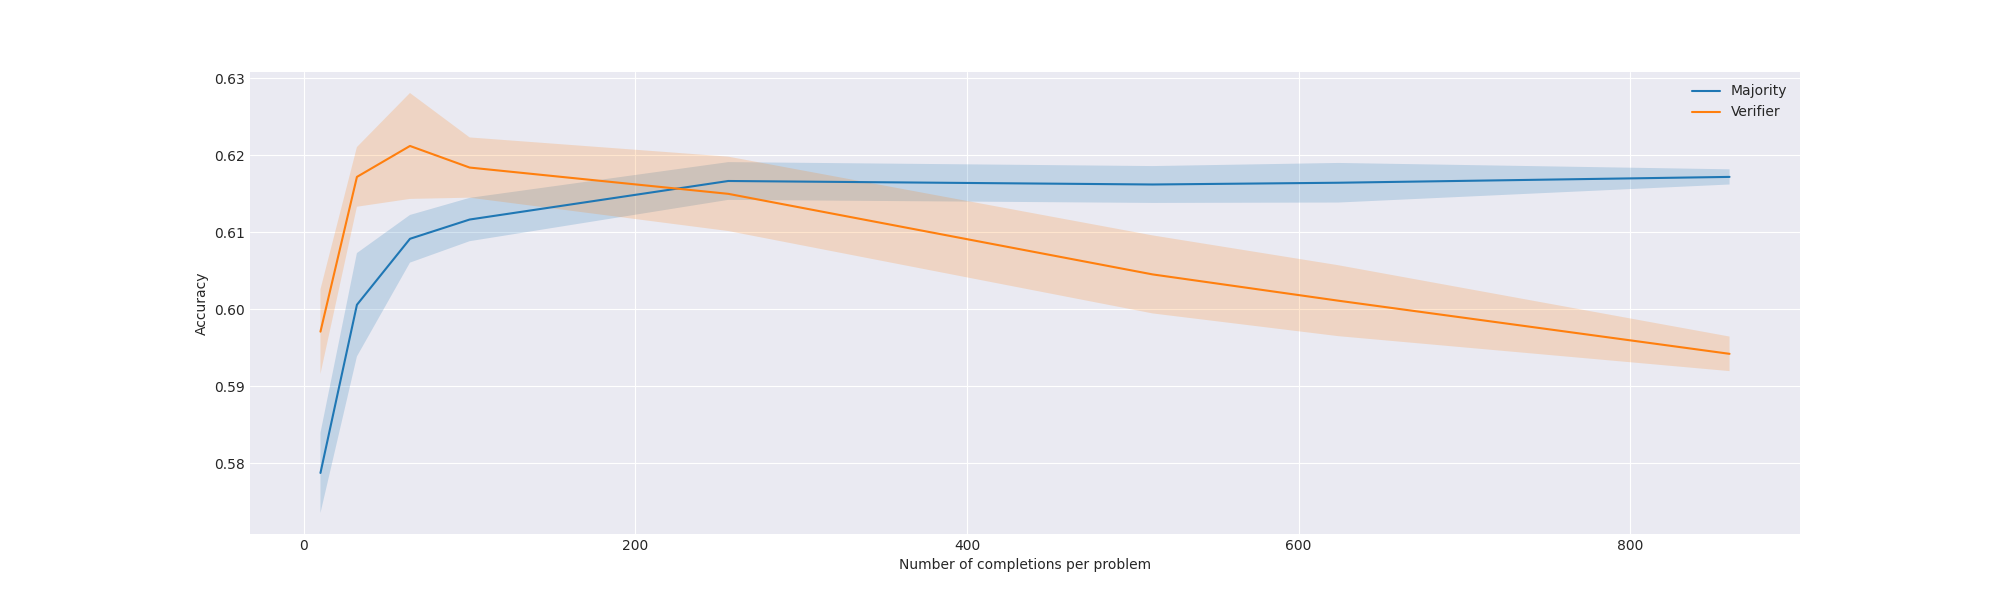
\includegraphics[width=\textwidth]{icml2023/figs/maj_vs_ver_large_completions.png}}
\caption{}
\label{}
\end{center}
\vskip -0.2in
\end{figure*}

\begin{figure}[ht]
% \vskip 0.2in
% \begin{center}
% \centerline{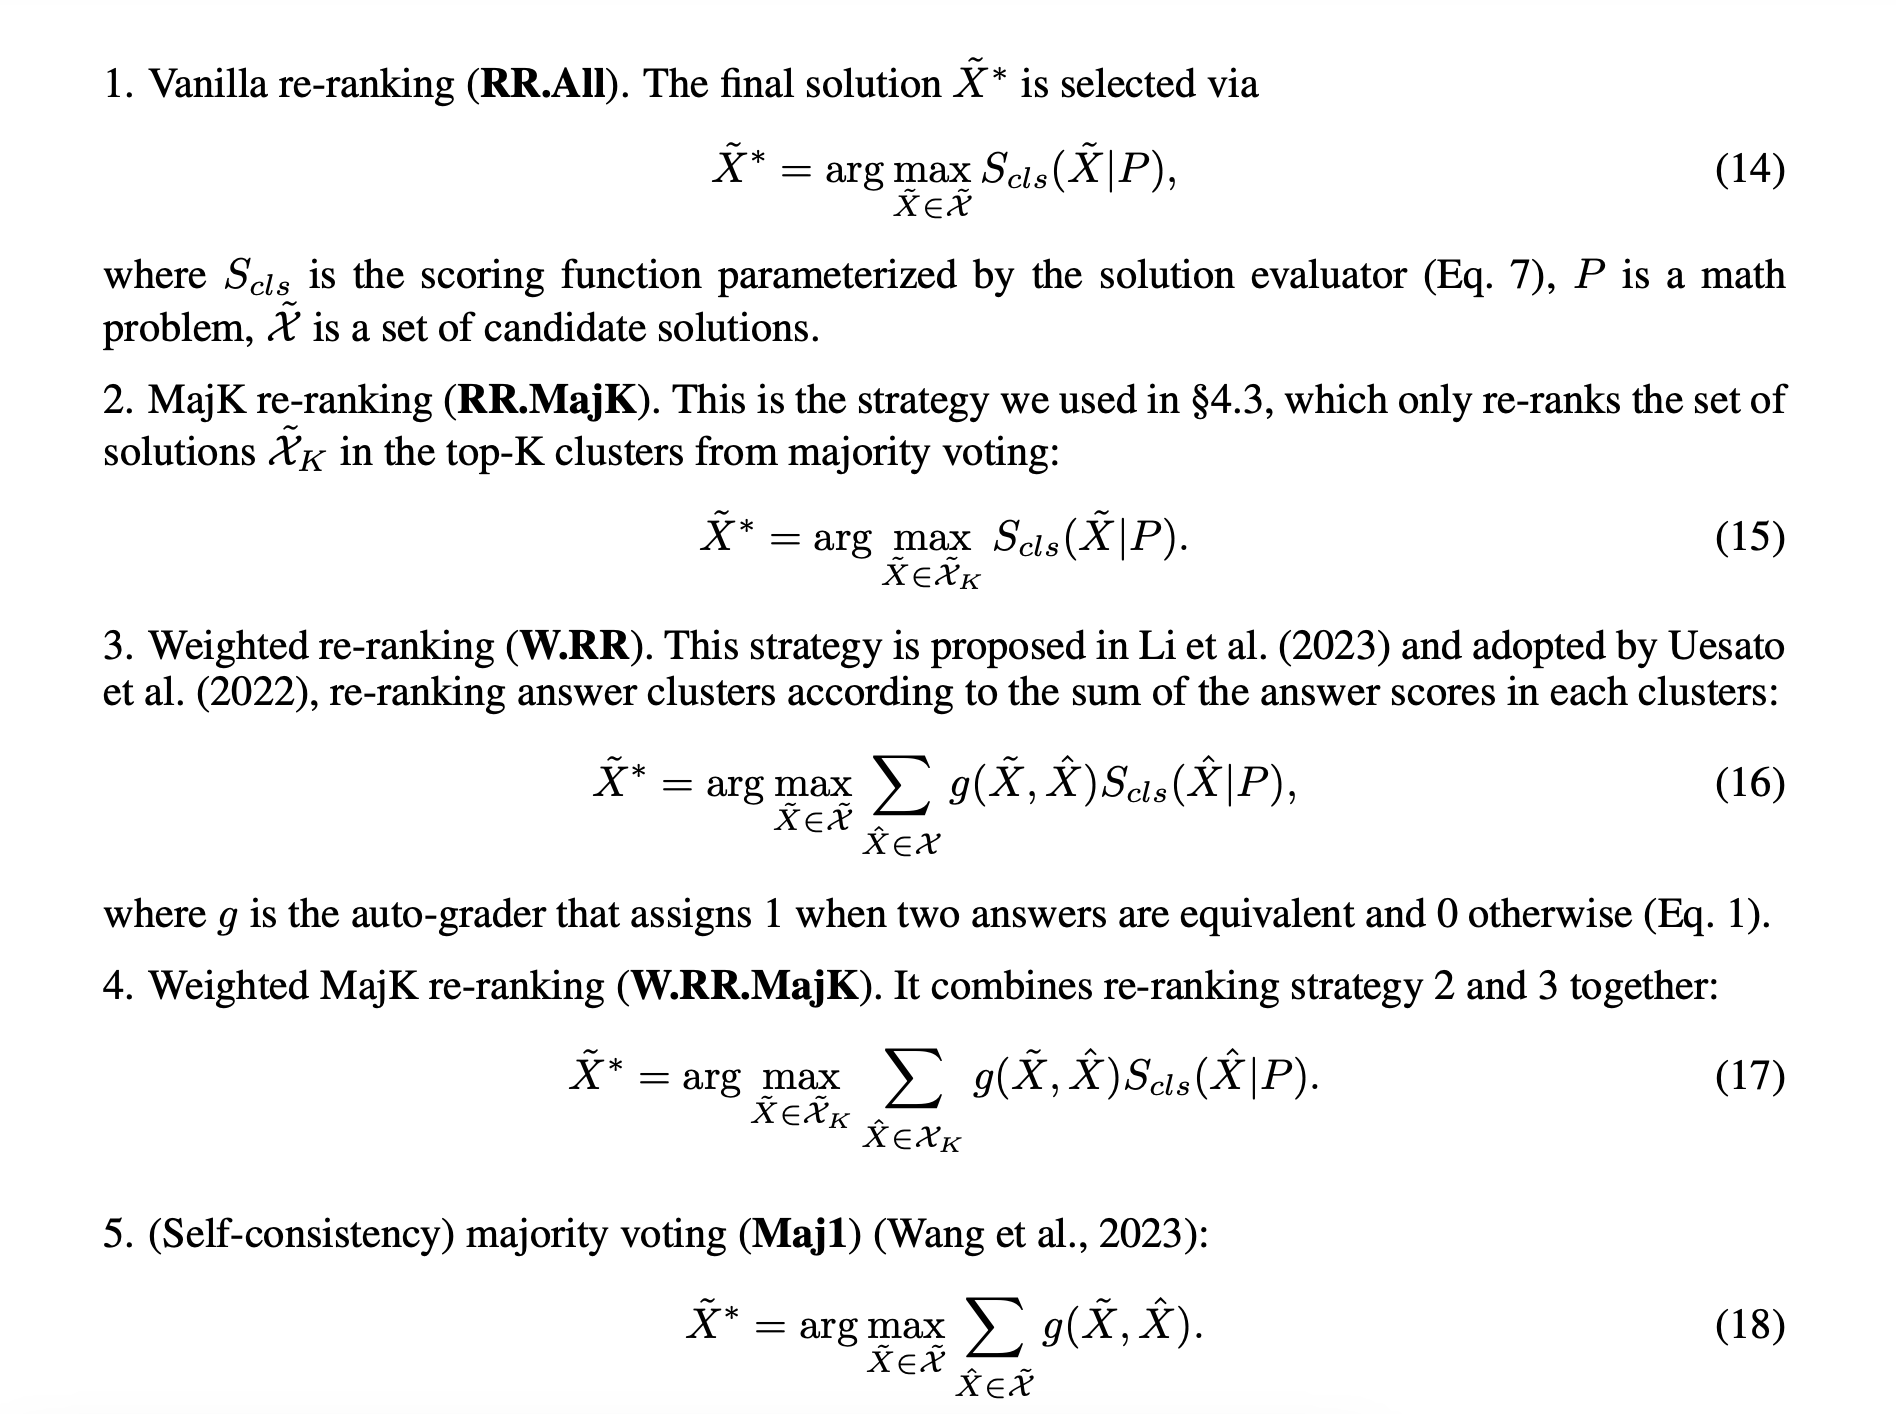
\includegraphics[width=\textwidth/2]{icml2023/figs/rerank_strategies.png}}
% \caption{Re-ranking strategies. We could do maj + verifier.}
% \end{center}
% \vskip -0.2in
% \end{figure}


\paragraph{Benchmark}
We plan to study our approach using the widely used Grade School Math (GSM8k) \citep{cobbe_training_2021} and ASDiv math word problems~\citep{miao_diverse_2020}. These datasets consist of logical, mathematical problems written in natural language and requiring multiple logical steps to answer. 

\begin{displayquote}
Leo's assignment was divided into three parts. He finished the first part of his assignment in 25 minutes. It took him twice as long to finish the second part. If he was able to finish his assignment in 2 hours, how many minutes did Leo finish the third part of the assignment?

\textbf{Solution} It took Leo 25 x 2 = 50 minutes to finish the second part of the assignment. Leo finished the first and second parts of the assignment in 25 + 50 = 75 minutes. He finished the entire assignment in 60 x 2 = 120 minutes. Therefore, it took Leo 120 - 75 = 45 minutes to finish the third part of the assignment.
\end{displayquote}


We also plan to evaluate on the MBPP benchmark~\citep{austin_program_2021} which consists of python coding questions and annotated solutions. We will experiment with scaling model sizes, different original training data sizes, as well as varying the number of iterations. 


\begin{table}[t]
\caption{Comparison of Iter.1 performance between models trained with uniform sampling batch examples vs non-uniform sampling. Gen. and Ver. are trained for 4k and 8k updates respectively.}
\label{sample-table}
\vskip 0.15in
\begin{center}
\begin{small}
\begin{sc}
\begin{tabular}{lcccr}
\toprule
Mode & Ver. Acc & Maj. Acc & Best @ 1 \\
\midrule
Uniform & 51.25 & 48.98 & 36.39\\
Non-uniform & 50.26 & 48.06 & 36.54 \\
\bottomrule
\end{tabular}
\end{sc}
\end{small}
\end{center}
\vskip -0.1in
\end{table}



\subsection{Code Results}
\begin{table*}[t]
\caption{MBPP Iteration Results Temperature 1}
\label{sample-table}
\vskip 0.15in
\begin{center}
\begin{small}
\begin{sc}
\begin{tabular}{llcccr}
\toprule
Generator & Verifier & Ver. Acc & Pass @ 10 & Pass @ 1 \\
\midrule
Base code llama7b. & - &  &  & 33.6 \\
\midrule
SFT.1 N=3x16 & Ver.1 N=3x16 & 48.4 & 65.60 & 37.79\\
\midrule
SFT.1 & Ver.1 &  &  &  \\
SFT.2 & Ver.2 &  &  &  \\
% cap32 below
% SFT.3 & Ver.3  & 51.8 & 67.88 & 46.41  \\ 
SFT.3 & Ver.3  & 53.8 & 68.06 & 46.11  \\ 

\bottomrule
\end{tabular}
\end{sc}
\end{small}
\end{center}
\vskip -0.1in
\end{table*}

\begin{table*}[t]
\caption{HumanEval Iteration Results Temperature 1}
\label{sample-table}
\vskip 0.15in
\begin{center}
\begin{small}
\begin{sc}
\begin{tabular}{llcccr}
\toprule
Generator & Verifier & Ver. Acc & Pass @ 10 & Pass @ 1 \\
\midrule
Base code llama7b. & - &  &  55.83 & 21.72\\
\midrule
SFT.1 N=3x16 & Ver.1 N=3x16 & 42.68 & 60.22 & 26.71 \\
% \midrule
SFT.3 & Ver.3  & 47.56 & 68.92 & 35.56  \\ 

\bottomrule
\end{tabular}
\end{sc}
\end{small}
\end{center}
\vskip -0.1in
\end{table*}



\begin{table*}[t]
\caption{Iteration Results for GSM8K}
\label{sample-table}
\vskip 0.15in
\begin{center}
\begin{small}
\begin{sc}
\begin{tabular}{llcccr}
\toprule
Generator & Verifier & Ver. Acc & Pass @ 10 & Pass @ 1 \\
\midrule
SFT Orig. & Ver.1 &  &  &  \\
\midrule
SFT.1 N=3x16 & Ver.1 N=3x16 & 58.22 & 73.27 & 38.11 \\
\midrule
SFT.1 & Ver.1 &  &  &  \\
SFT.2 & Ver.2 &  &  &  \\
SFT.3 & Ver.3 & 63.00 & 79.13 & 47.21 \\
\bottomrule
\end{tabular}
\end{sc}
\end{small}
\end{center}
\vskip -0.1in
\end{table*}


\begin{table}[t]
\caption{How important are negative samples for the Verifier?}
\label{sample-table}
\vskip 0.15in
\begin{center}
\begin{small}
\begin{sc}
\begin{tabular}{lcccr}
\toprule
\backslashbox{Ver.}{Gen.} & Filter Pos & C/O & Full \\
\midrule
Filter Pos - C/O Neg  & 61.94 & & 62.47\\
Filter Pos - Fill Neg  & 61.41& & 61.71\\
Filter Pos - Full Neg  & 61.18& & 62.62\\
Full Pos - Full Neg  & 61.64& & 63.0\\
\midrule
Pass @ 1 & 46.69 & & 47.21 \\
Pass @ 10 & 77.79 &  & 79.13\\
\bottomrule
\end{tabular}
\end{sc}
\end{small}
\end{center}
\vskip -0.1in
\end{table}


\begin{table}[t]
\caption{LLaMA 13B results on GSM8K}
\label{sample-table}
\vskip 0.15in
\begin{center}
\begin{small}
\begin{sc}
\begin{tabular}{lcccr}
\toprule
Mode & Ver. Acc & Maj. Acc & Best @ 1 \\
\midrule
Baseline  & 69.74 & 65.58 & 54.21\\
V-star & 72.63 & 67.62 & 59.05 \\
\bottomrule
\end{tabular}
\end{sc}
\end{small}
\end{center}
\vskip -0.1in
\end{table}

\begin{table}[t]
\caption{LLaMA 13B results on MBPP}
\label{sample-table}
\vskip 0.15in
\begin{center}
\begin{small}
\begin{sc}
\begin{tabular}{lcccr}
\toprule
Mode & Ver. Acc & Pass @ 10 & Pass @ 1 \\
\midrule
Baseline  & 55.4 & 73.77 & 48.85\\
V-star & 58.6 & 73.48 & 50.96 \\
\bottomrule
\end{tabular}
\end{sc}
\end{small}
\end{center}
\vskip -0.1in
\end{table}

\begin{table}[t]
\caption{Performance on a subset of MATH test data including Level 1,2 from Algebra, Intermediate Algebra, Counting \& Probability, Prealgebra, 
Number Theory}
\label{sample-table}
\vskip 0.15in
\begin{center}
\begin{small}
\begin{sc}
\begin{tabular}{lcccr}
\toprule
Mode & Ver. Acc & Maj. Acc & Best @ 1 \\
\midrule
Baseline  & 12.74 & 16.77 & 11.46\\
V-star & 16.14 & 18.26 & 14.86 \\
\bottomrule
\end{tabular}
\end{sc}
\end{small}
\end{center}
\vskip -0.1in
\end{table}

\begin{table}[t]
\caption{Comparison of using \textit{perplexity} vs \textit{reward} from the DPO trained verifier as ranking}
\label{sample-table}
\vskip 0.15in
\begin{center}
\begin{small}
\begin{sc}
\begin{tabular}{lc}
\toprule
Mode & Ver. Acc \\
\midrule
$ppl \textit{ under policy}$  & 50.87 \\
$logp(\textit{policy})$ - $logp(\textit{ref})$ & 50.26\\
\bottomrule
\end{tabular}
\end{sc}
\end{small}
\end{center}
\vskip -0.1in
\end{table}


\begin{table}[t]
\caption{Filtering generations for Iteration 3 based. Comparing a Cutoffs of sizes 10 and 16 to filtering with the verifier from Iteration 2.}
\label{sample-table}
\vskip 0.15in
\begin{center}
\begin{small}
\begin{sc}
\begin{tabular}{lcccr}
\toprule
Mode & Ver. Acc & Maj. Acc & Best @ 1 \\
\midrule
Full Data  & 56.48 & 57.32 & 45.49 \\
\midrule
Cutoff 10  & 53.98 & 55.27 & 43.21\\
Cutoff 16 & 58.83 & 56.63 & 45.79 \\
\midrule
Ver.  & 56.41 & 56.56 & 45.11 \\
\bottomrule
\end{tabular}
\end{sc}
\end{small}
\end{center}
\vskip -0.1in
\end{table}

% The training objective for our DPO based verifiers is 
% \begin{multline}
%     \mathcal{L}_{\text{VER}}(\pi_{\theta}; \pi_{\text{ref}}) = \\
%     - \E_{(x, \hat{r}_w, \hat{r}_l) \sim \mathcal{D}_{\text{VER}}} \left[ \log \sigma \left( \hat{g}_\theta(x,\hat{r}_w) -  \hat{g}_\theta(x,\hat{r}_l) \right) \right]
% \end{multline}


% \begin{table*}[t]
% \caption{Comparison of  self-improvement and verification-based methods, showing the data used to train the generator and verifier (if applicable), and whether or not the method is iterative.}
% \label{tab:bootstrap_methods}
% \begin{center}
% % \begin{footnotesize}
% \begin{sc}
% \footnotesize
% \begin{tabular}{@{}lllr}
% \toprule
% Method & Generator Data & Verifier Data & Iterative \\
% \midrule
% SFT & $\mathcal{D}_{\text{SFT}}$  & \xmark & \xmark \\
% Verification & $\mathcal{D}_{\text{SFT}}$  & $\mathcal{D}_{\text{SFT}}$ $\cup$ Generated & \xmark \\
% STaR & $\text{Correct Generated}_{t-1}$ & \xmark & \cmark \\
% RFT~(\stardag[1 iter]) &  $\mathcal{D}_{\text{SFT}}$ $\cup$ Correct Generated & \xmark & \xmark \\
% \stardag & $\mathcal{D}_{\text{SFT}}$ $\cup$ $\text{Correct Generated}_{<t}$ & \xmark & \cmark \\\midrule
% \vstar{} [1 Iter] & $\mathcal{D}_{\text{SFT}}$ $\cup$ Correct Generated & $\mathcal{D}_{\text{SFT}}$ $\cup$  Generated & \xmark \\
% \textbf{\vstar{}} & $\boldsymbol{\mathcal{D}}_{\textbf{SFT}}$ $\boldsymbol{\cup}$ $\textbf{Correct Generated}_{\boldsymbol{<t}}$ & $\boldsymbol{\mathcal{D}}_{\textbf{SFT}}$ $\boldsymbol{\cup}$ $\textbf{Generated}_{\boldsymbol{<t}}$ & \textbf{\cmark} \\
% \bottomrule
% \end{tabular}
% \end{sc}
% % \end{footnotesize}
% \end{center}
% \vskip -0.1in
% \end{table*}


\begin{figure*}[ht]
\vskip 0.2in
\begin{center}
\centerline{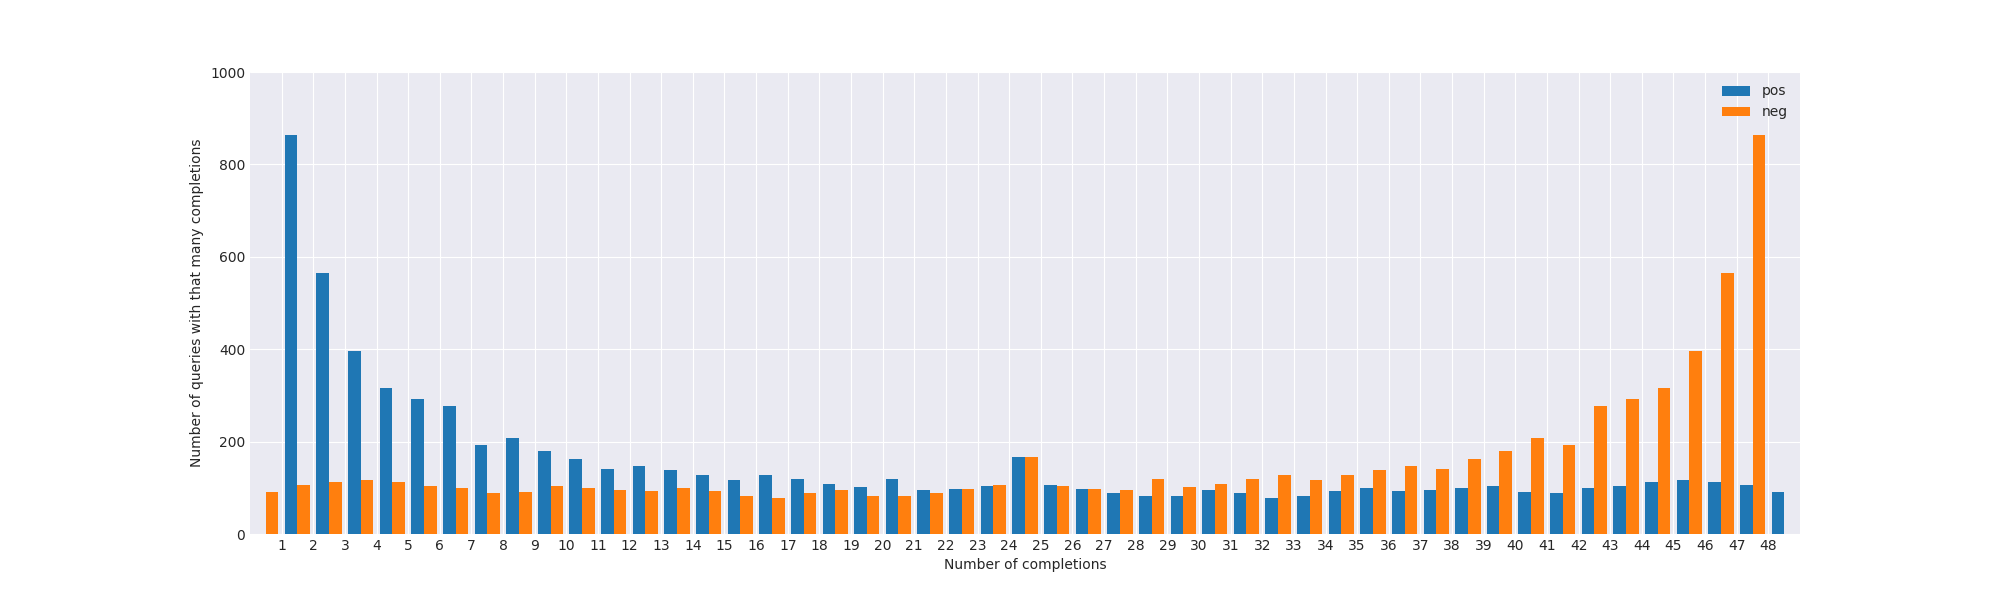
\includegraphics[width=\textwidth]{icml2023/figs/N3x16_FF_v5.png}}
\caption{Histogram of distribution of positive and negative completions for iteration one with N=3x16 completions per query}
\label{icml-historical}
\end{center}
\vskip -0.2in
\end{figure*}

\begin{figure*}[ht]
\vskip 0.2in
\begin{center}
\centerline{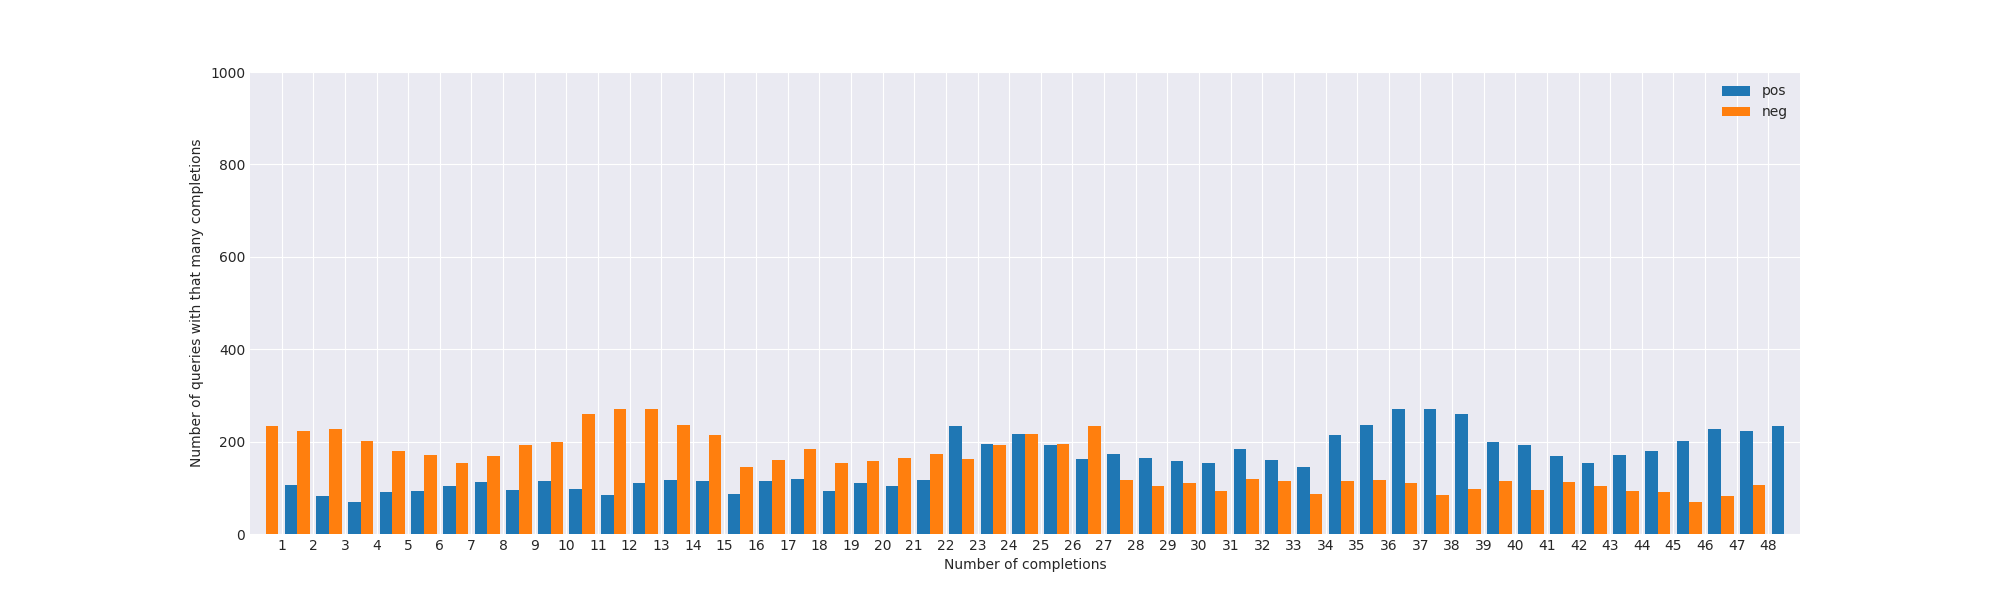
\includegraphics[width=\textwidth]{icml2023/figs/iter3_N16_FF_v5.png}}
\caption{Histogram of distribution of positive and negative completions for iteration 3}
\label{icml-historical}
\end{center}
\vskip -0.2in
\end{figure*}


%%RA.1.26: This paper should be about explaining self-improvement approaches and their short-coming. Basically expanding these two abstract sentecnes:
% Common self-improvement approaches for large language models~(LLMs) iteratively fine-tune  LLMs on self-generated solutions to improve their problem-solving ability. However, these approaches discard the large amounts of incorrect solutions generated during this process.
Large language models~(LLMs) have demonstrated impressive performance on various tasks~\citep{DBLP:journals/corr/abs-2307-09288, openai2023gpt4}. However, LLMs often fall short on multi-step reasoning tasks, such as code-generation. To improve the reasoning performance of LLMs, several approaches exploit the ability of LLMs to produce solutions and check the correctness of these solutions during training, for example, using test cases for code generation. These self-improvement approaches, such as STaR \cite{DBLP:conf/nips/ZelikmanWMG22},  RFT~\citep{yuan2023scaling}, and ReST$^{EM}$~\citep{singh2023human}, improve LLMs by fine-tuning them on their self-generated solutions and optionally iteratively running this process.
However, all these approaches are data-inefficient in that they use \emph{only} correct solutions, and discard incorrect solutions, which is often a large portion of model-generated solutions, especially for challenging reasoning tasks. 


% To improve the models in this matter, researchers have proposed various prompting methods \cite{DBLP:conf/iclr/FuPSCK23, sordoni2023joint}, self-improvement techniques \cite{DBLP:conf/nips/ZelikmanWMG22, gulcehre2023reinforced, yuan2023scaling} and verification \cite{DBLP:journals/corr/abs-2110-14168, DBLP:journals/corr/abs-2305-20050, DBLP:journals/corr/abs-2312-08935}. 
